\begin{figure}%
    \centering
    \subfloat[Instância 0]{{
        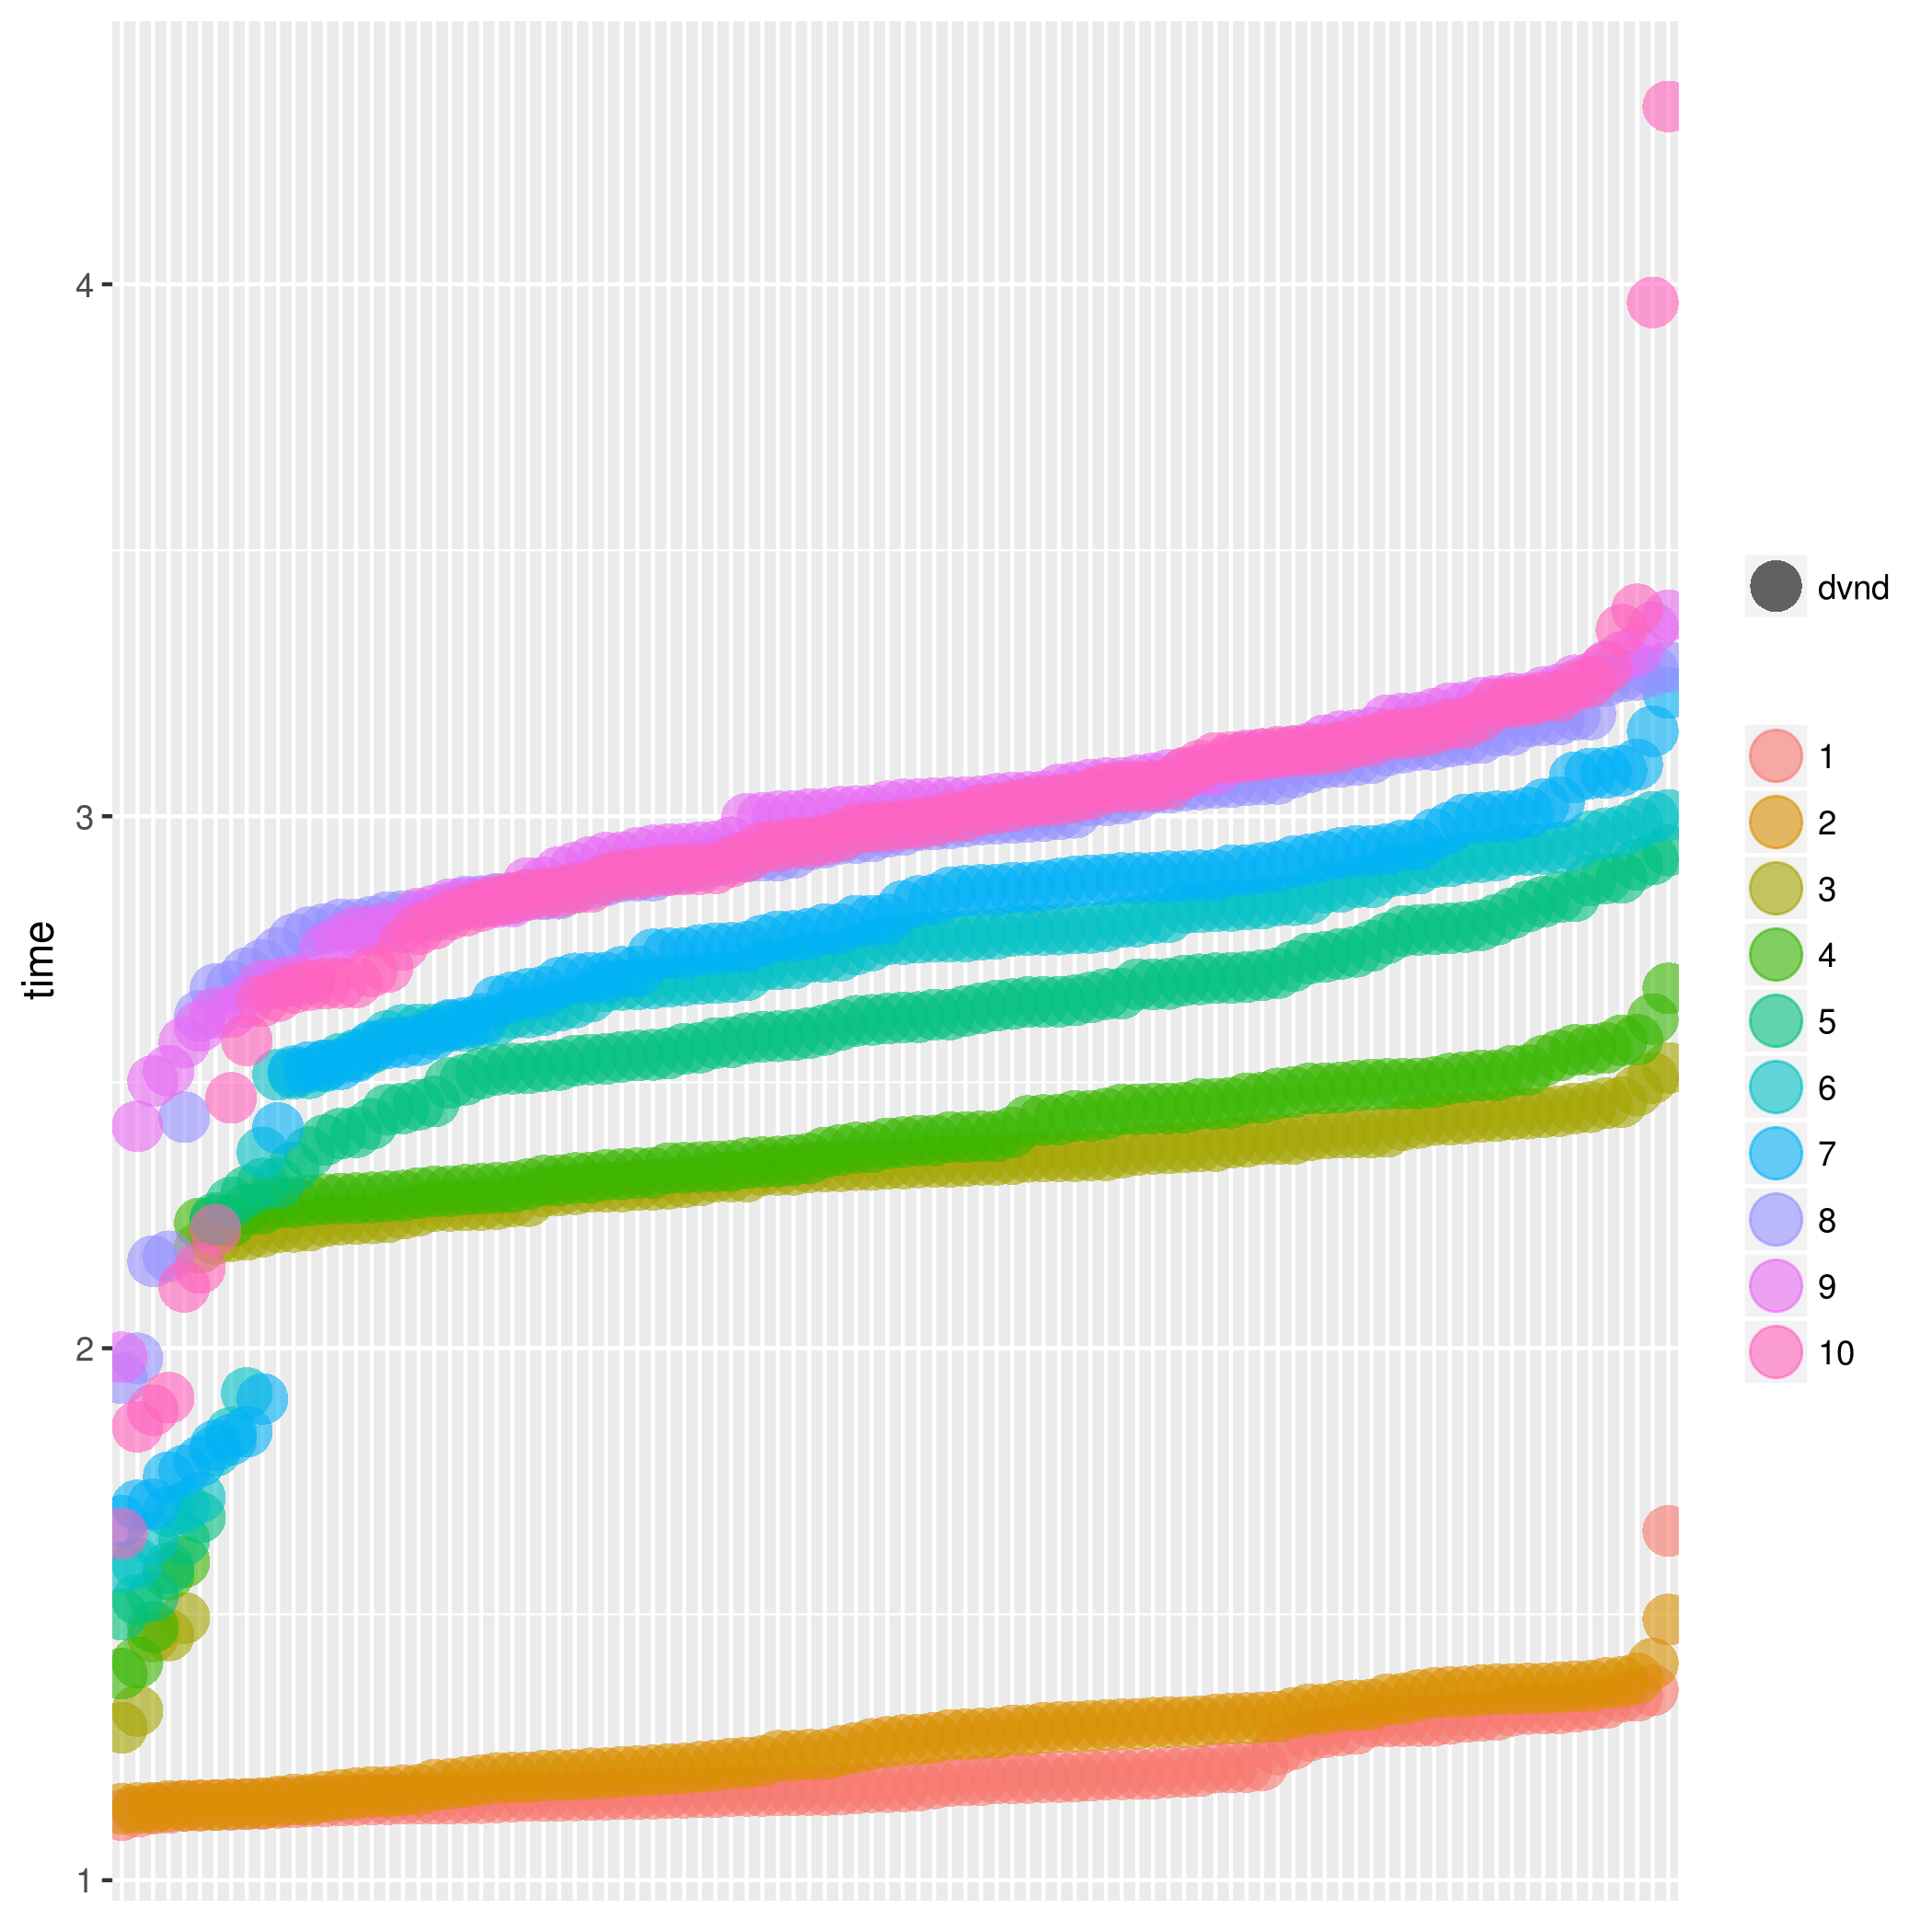
\includegraphics[scale=0.4]{figuras/dvnd/n1/time0.png}
        \label{fig:timeDvndRvnd_n1in0}
    }}%
    \qquad
    \subfloat[Instância 1]{{
        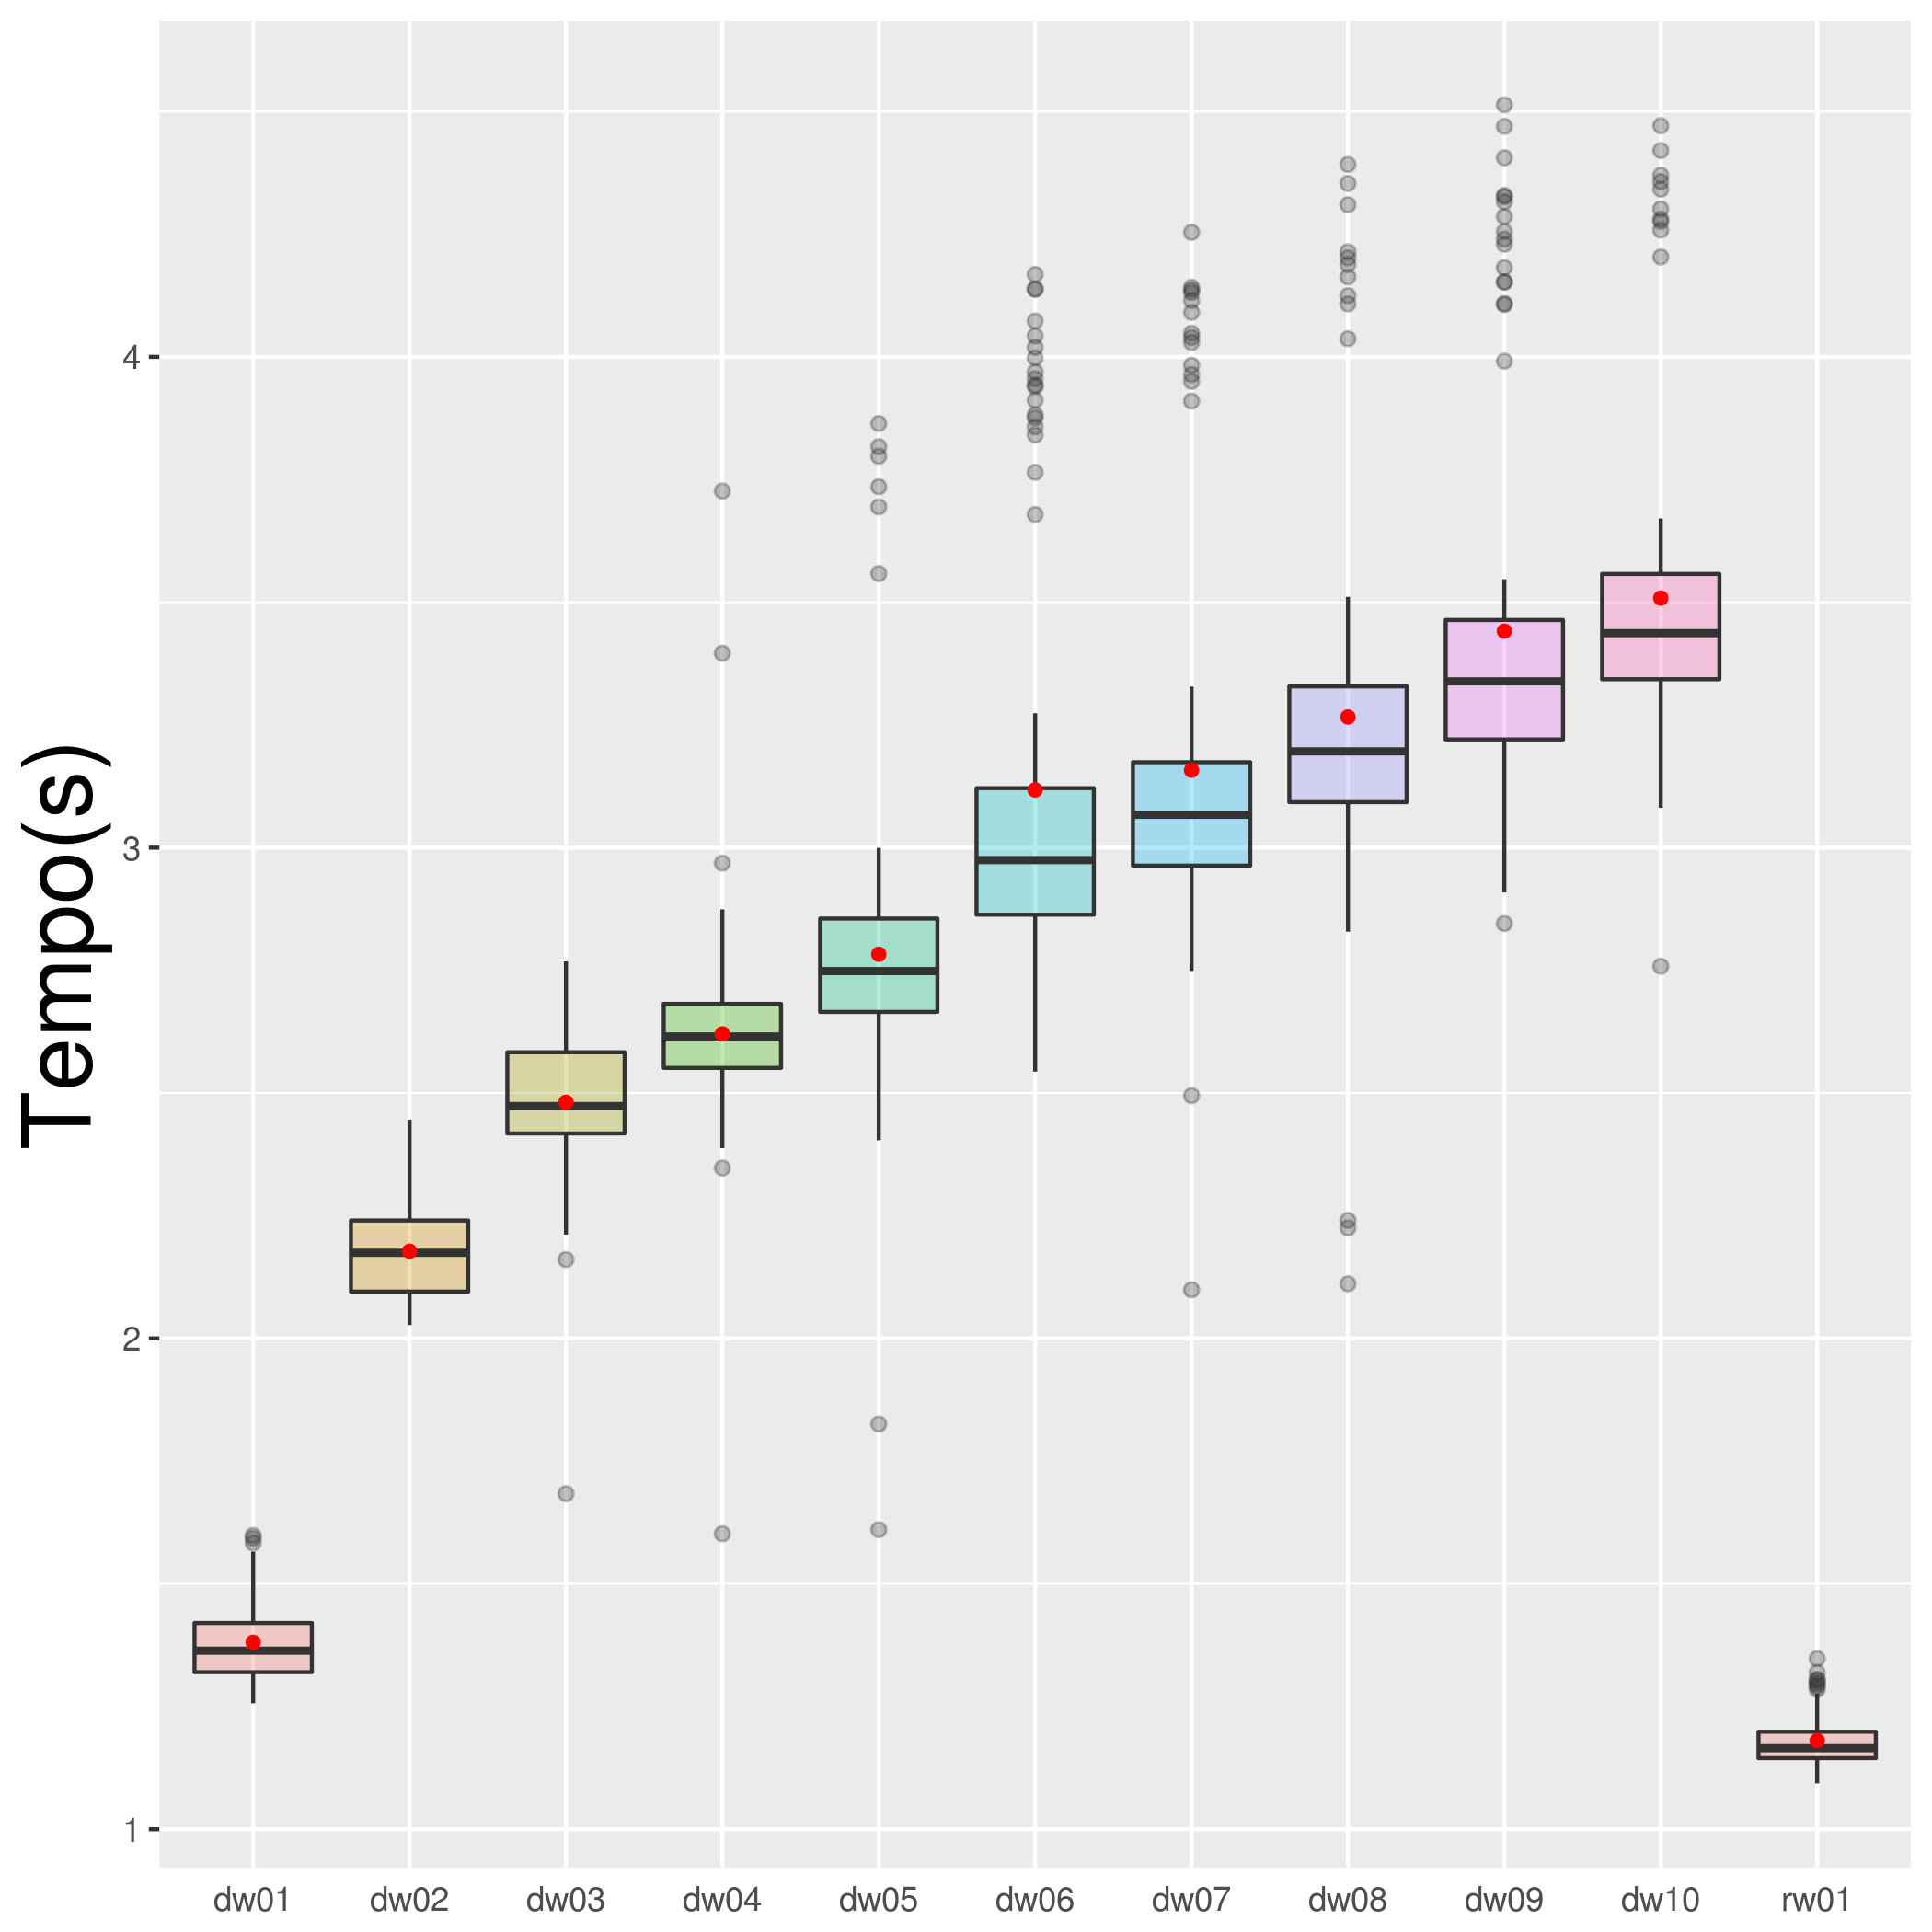
\includegraphics[scale=0.4]{figuras/dvnd/n1/time1.png}
        \label{fig:timeDvndRvnd_n1in1}
    }}%
    \caption{Tempos DVND e RVND das instâncias 0 e 1 para $n=1$.}%
    \label{fig:timeDvndRvnd_n1in0_1}%
\end{figure}

\begin{figure}%
    \centering
    \subfloat[Instância 2]{{
        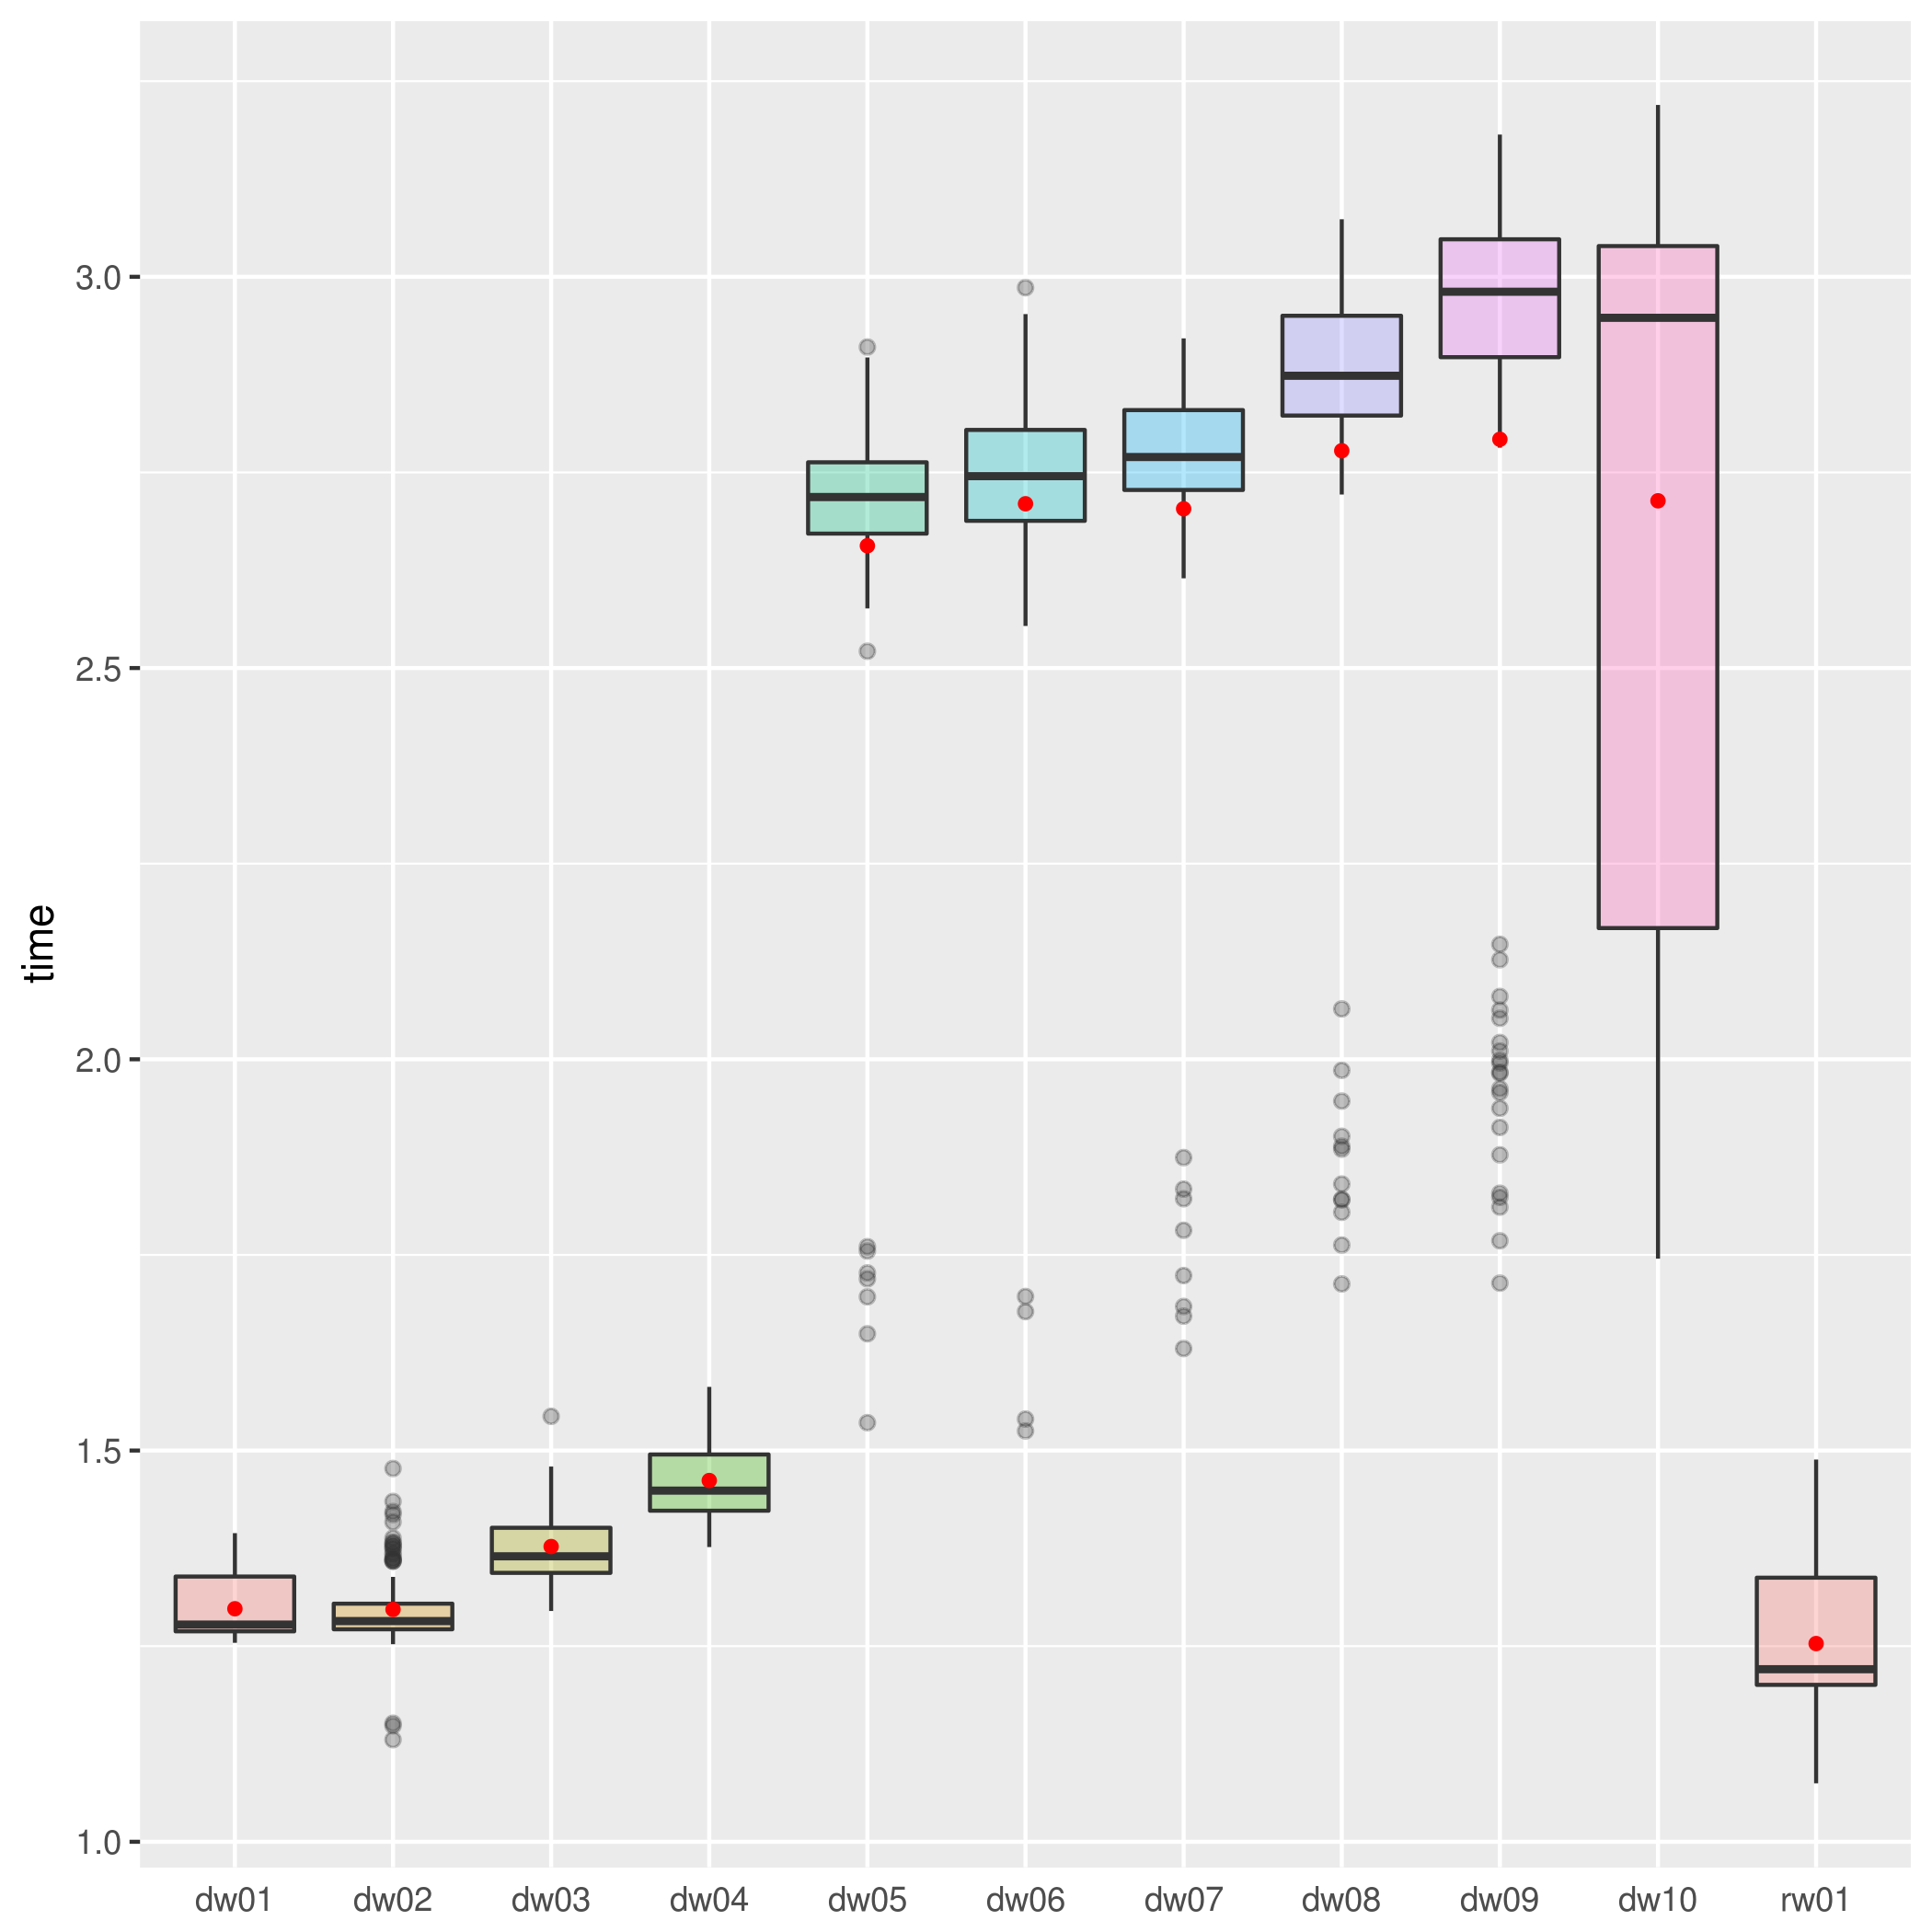
\includegraphics[scale=0.4]{figuras/dvnd/n1/time2.png}
        \label{fig:timeDvndRvnd_n1in2}
    }}%
    \qquad
    \subfloat[Instância 3]{{
        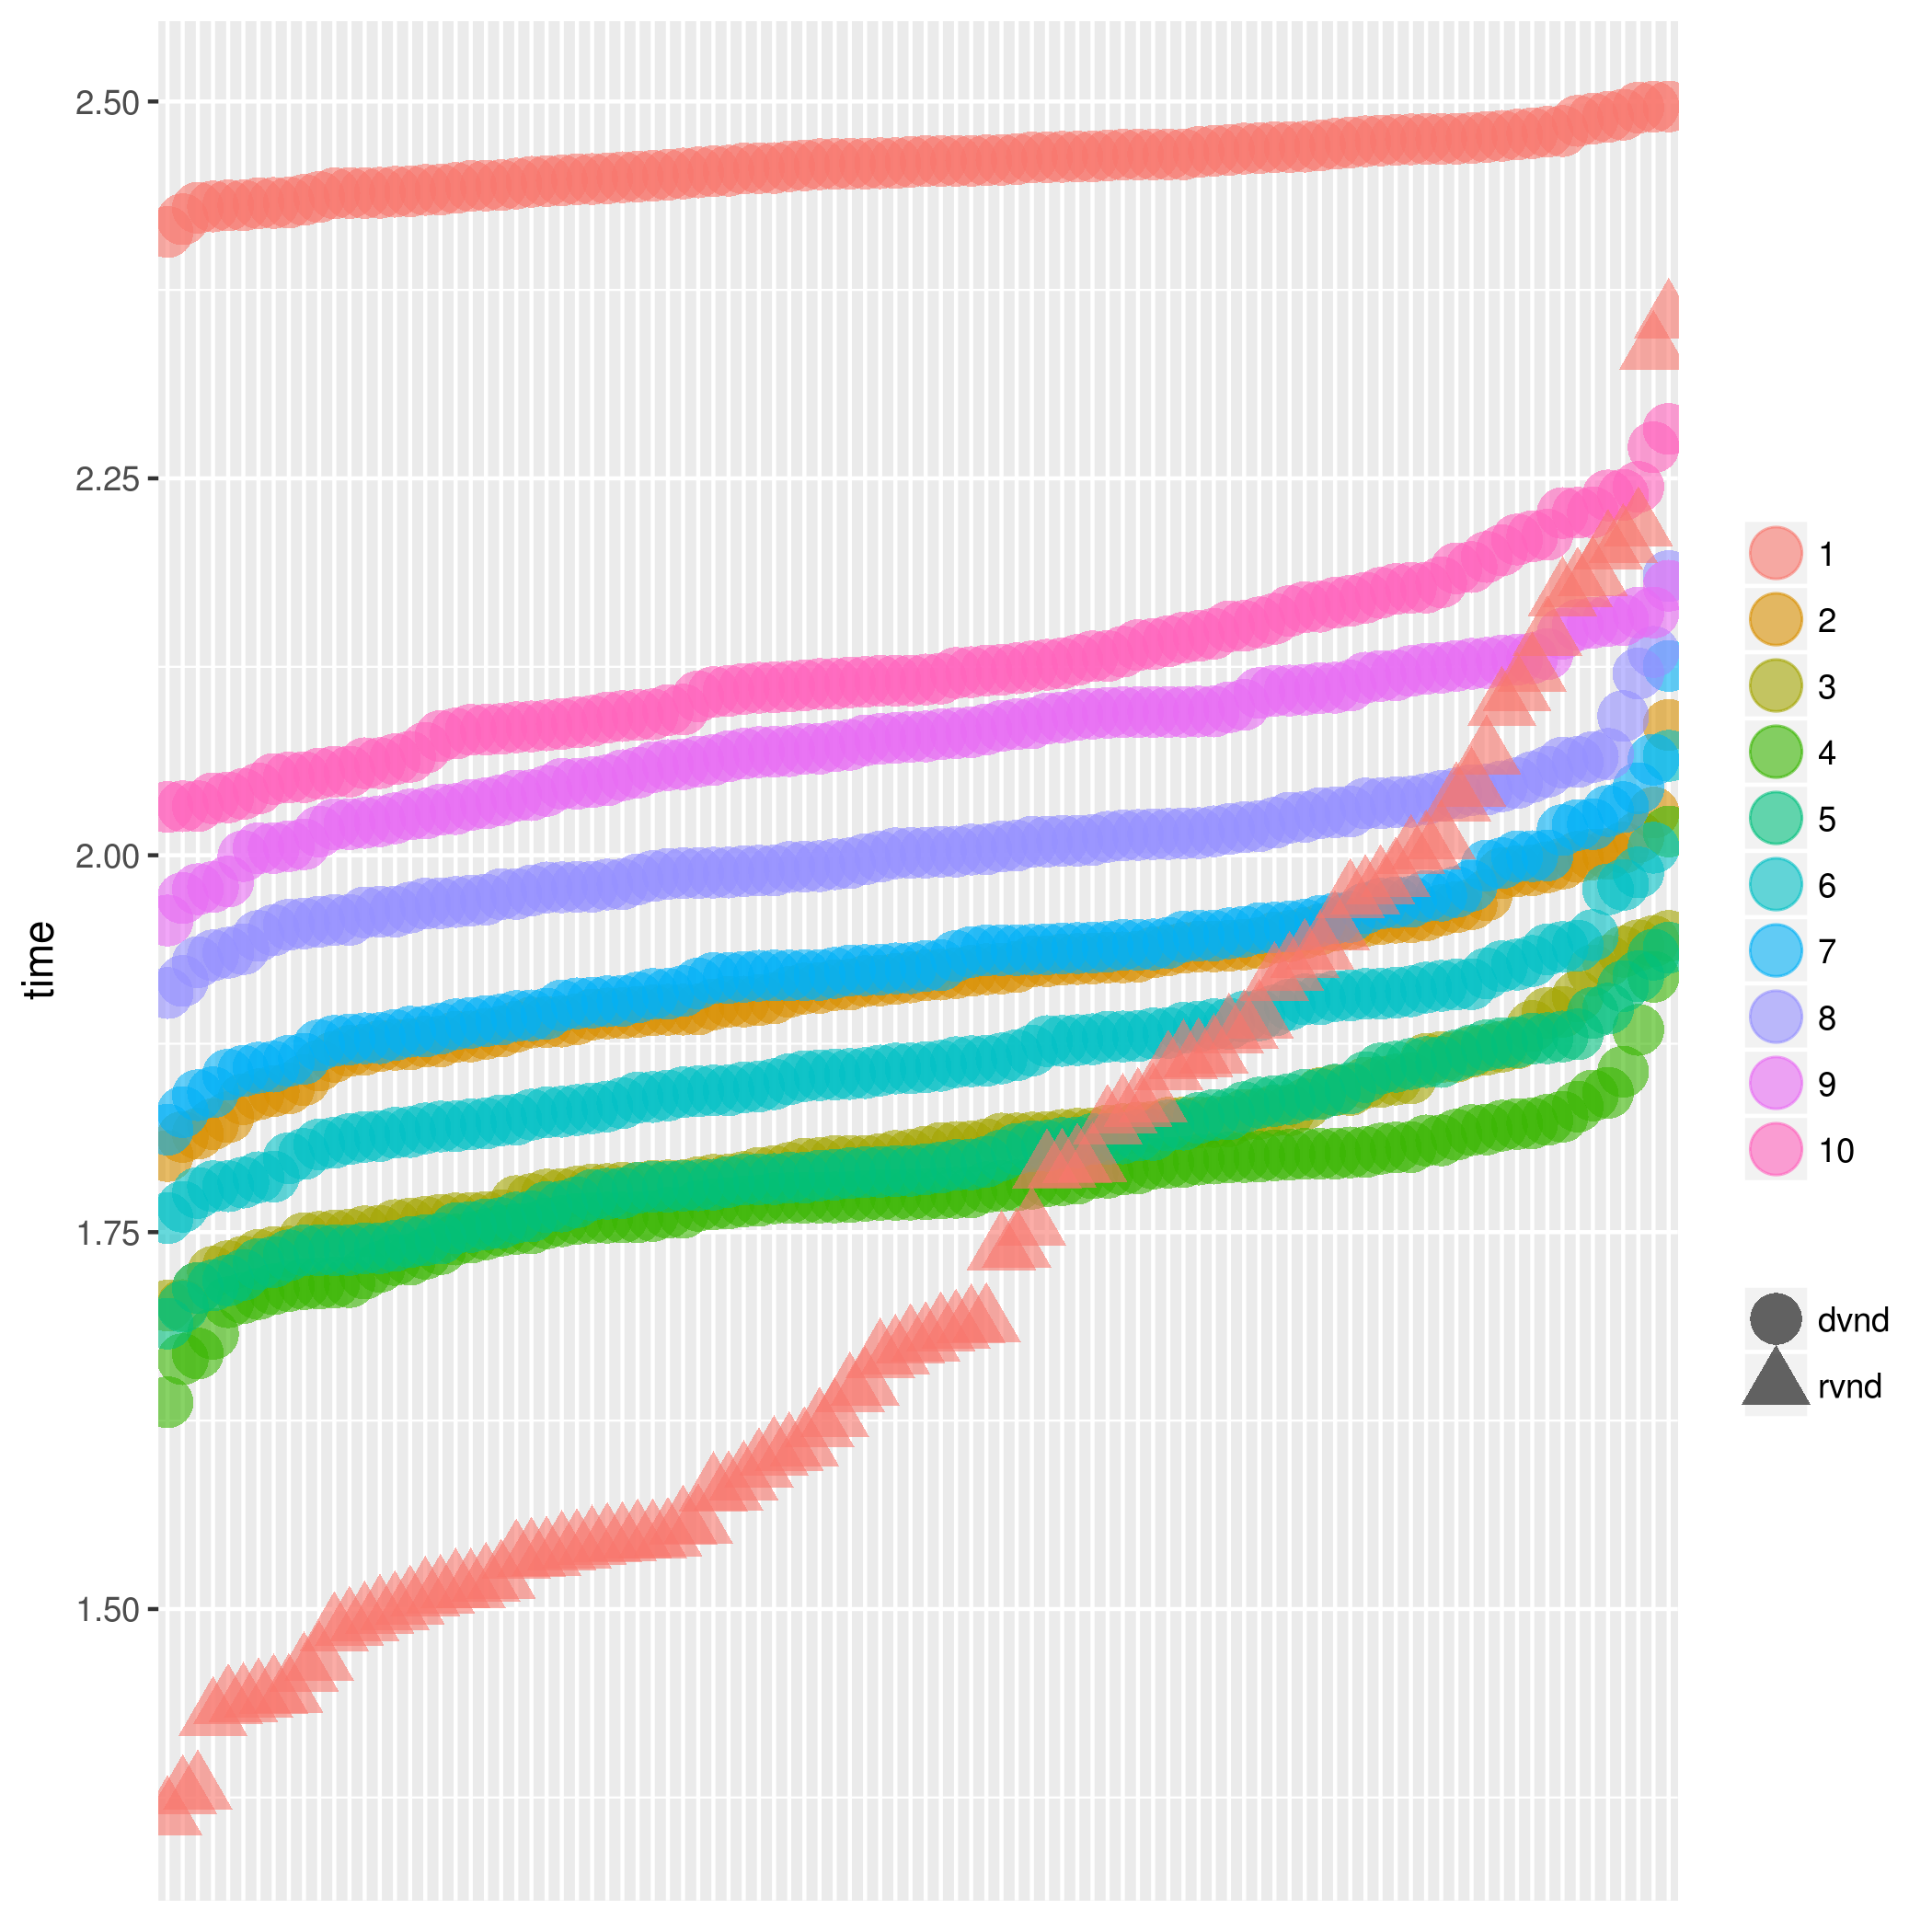
\includegraphics[scale=0.4]{figuras/dvnd/n1/time3.png}
        \label{fig:timeDvndRvnd_n1in3}
    }}%
    \caption{Tempos DVND e RVND das instâncias 2 e 3 para $n=1$.}%
    \label{fig:timeDvndRvnd_n1in2_3}%
\end{figure}

\begin{figure}%
    \centering
    \subfloat[Instância 4]{{
        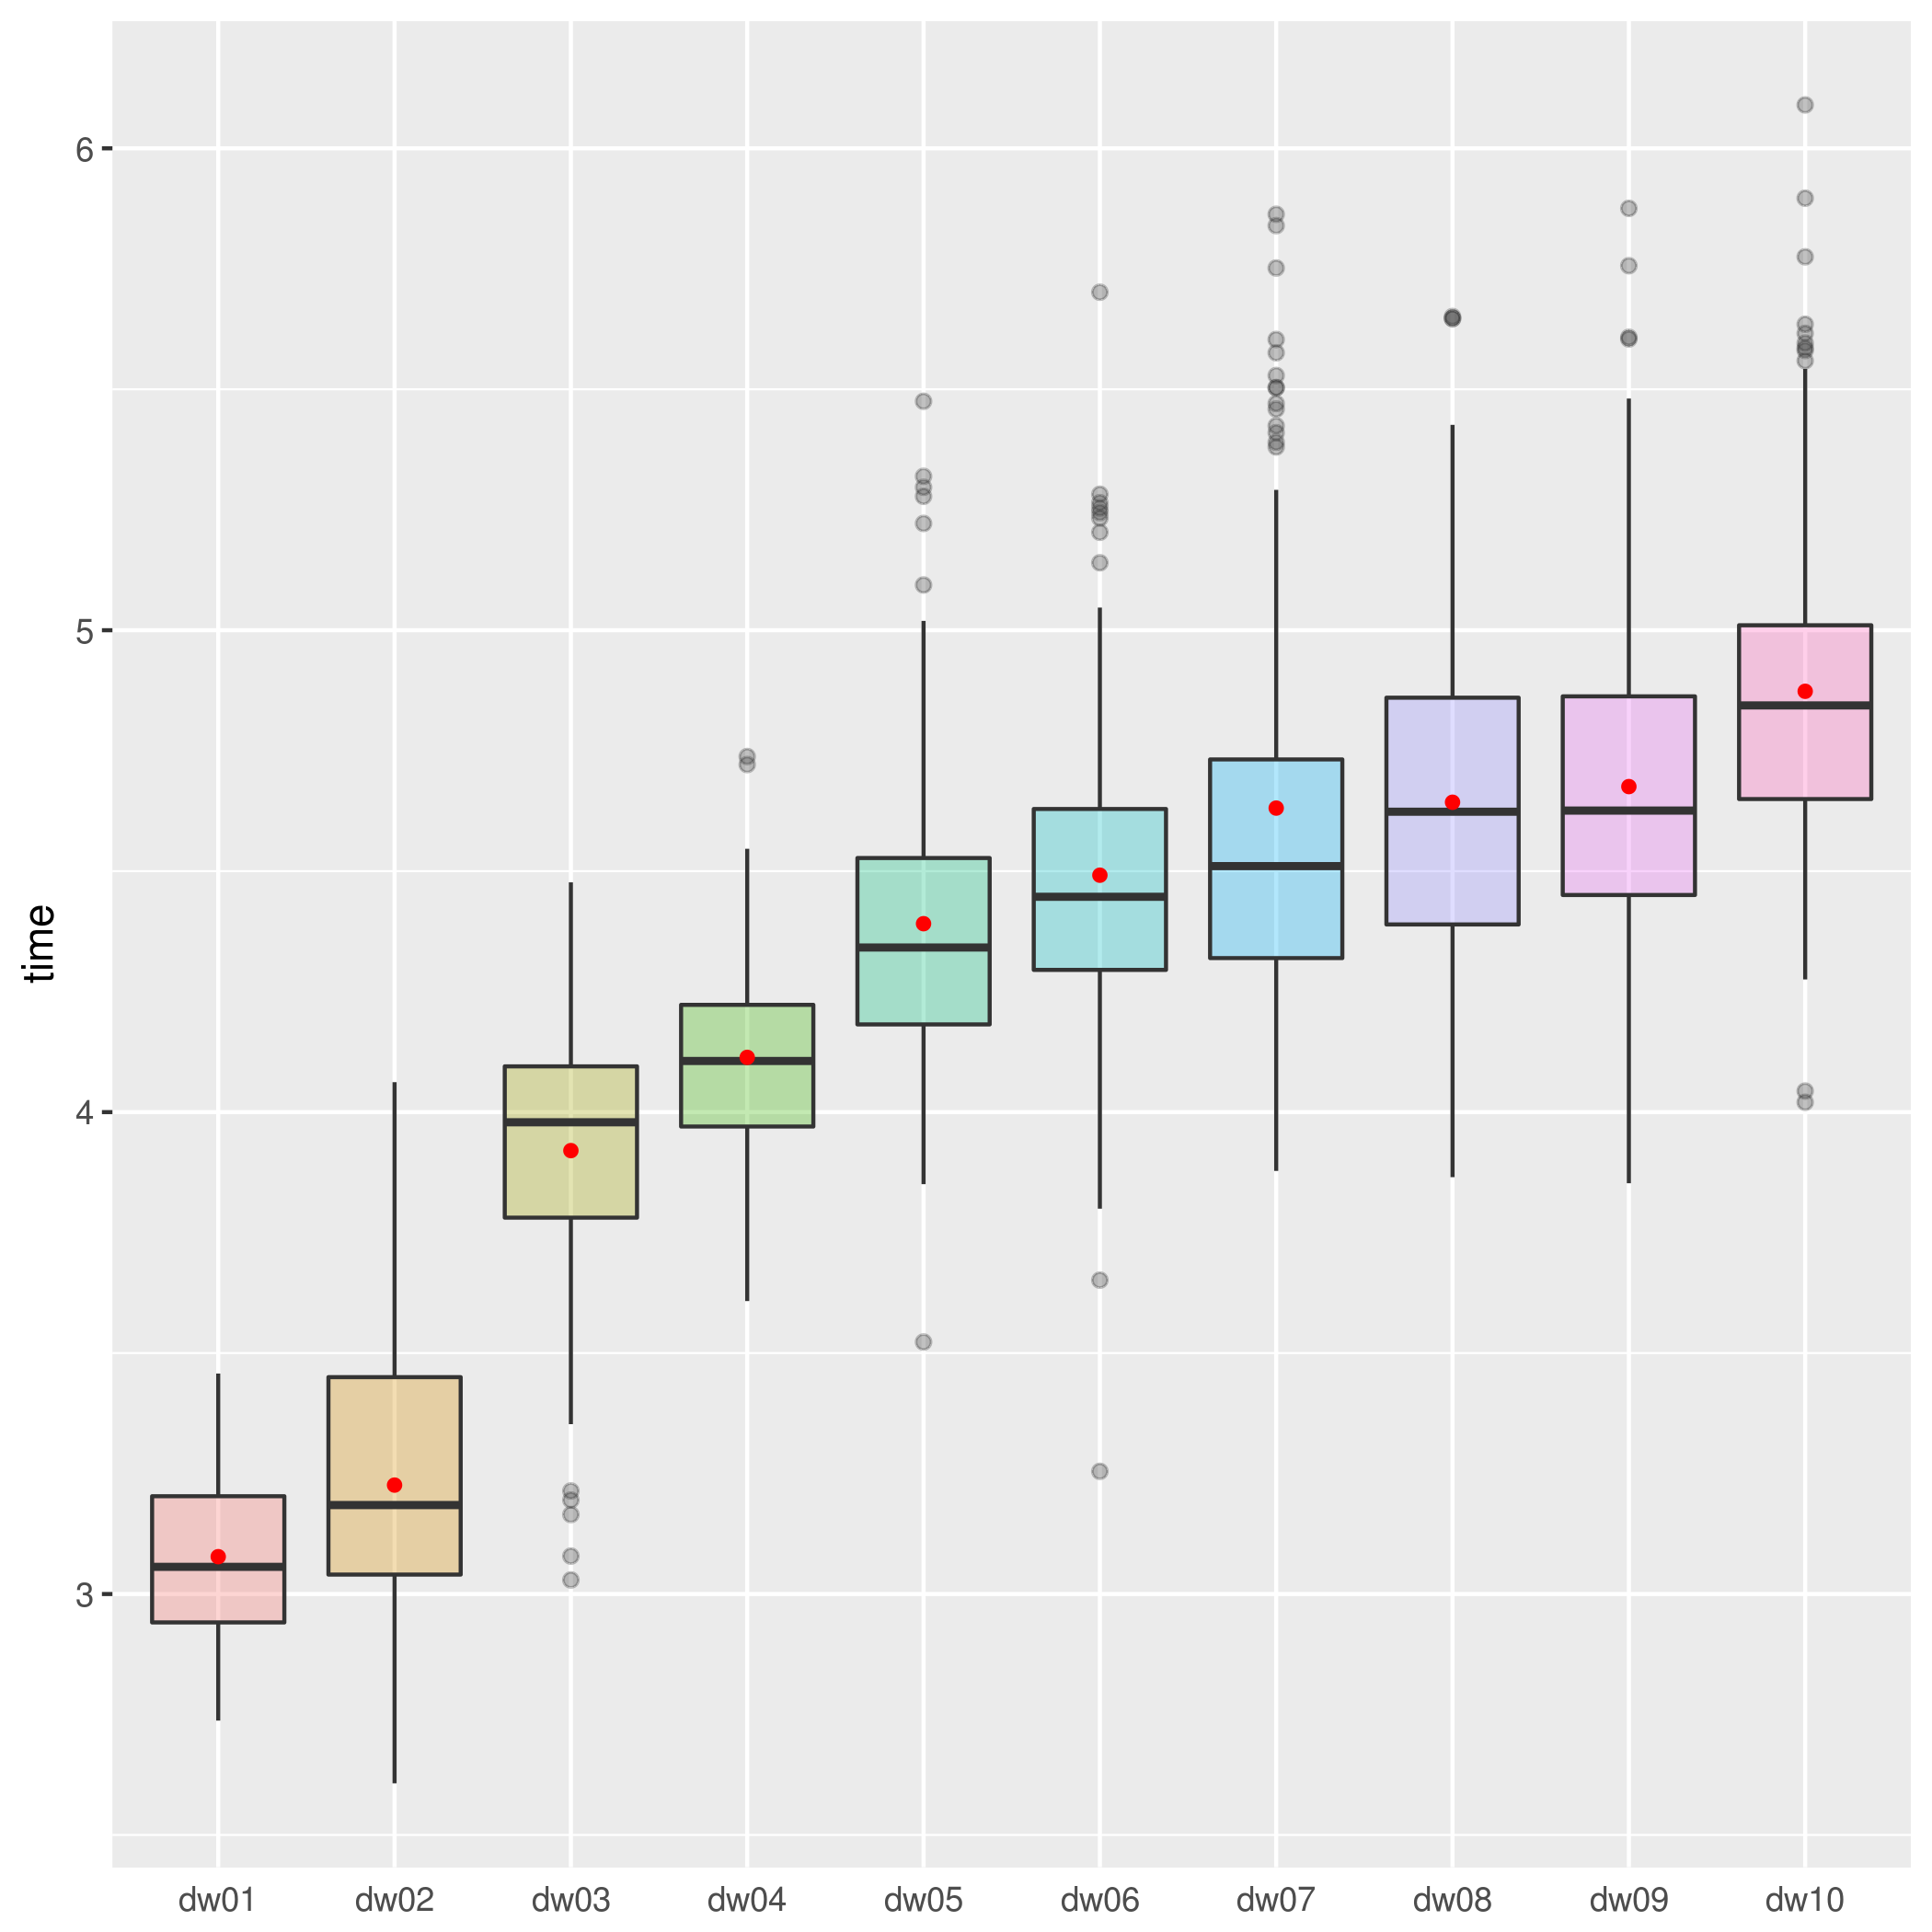
\includegraphics[scale=0.4]{figuras/dvnd/n1/time4.png}
        \label{fig:timeDvndRvnd_n1in4}
    }}%
    \qquad
    \subfloat[Instância 5]{{
        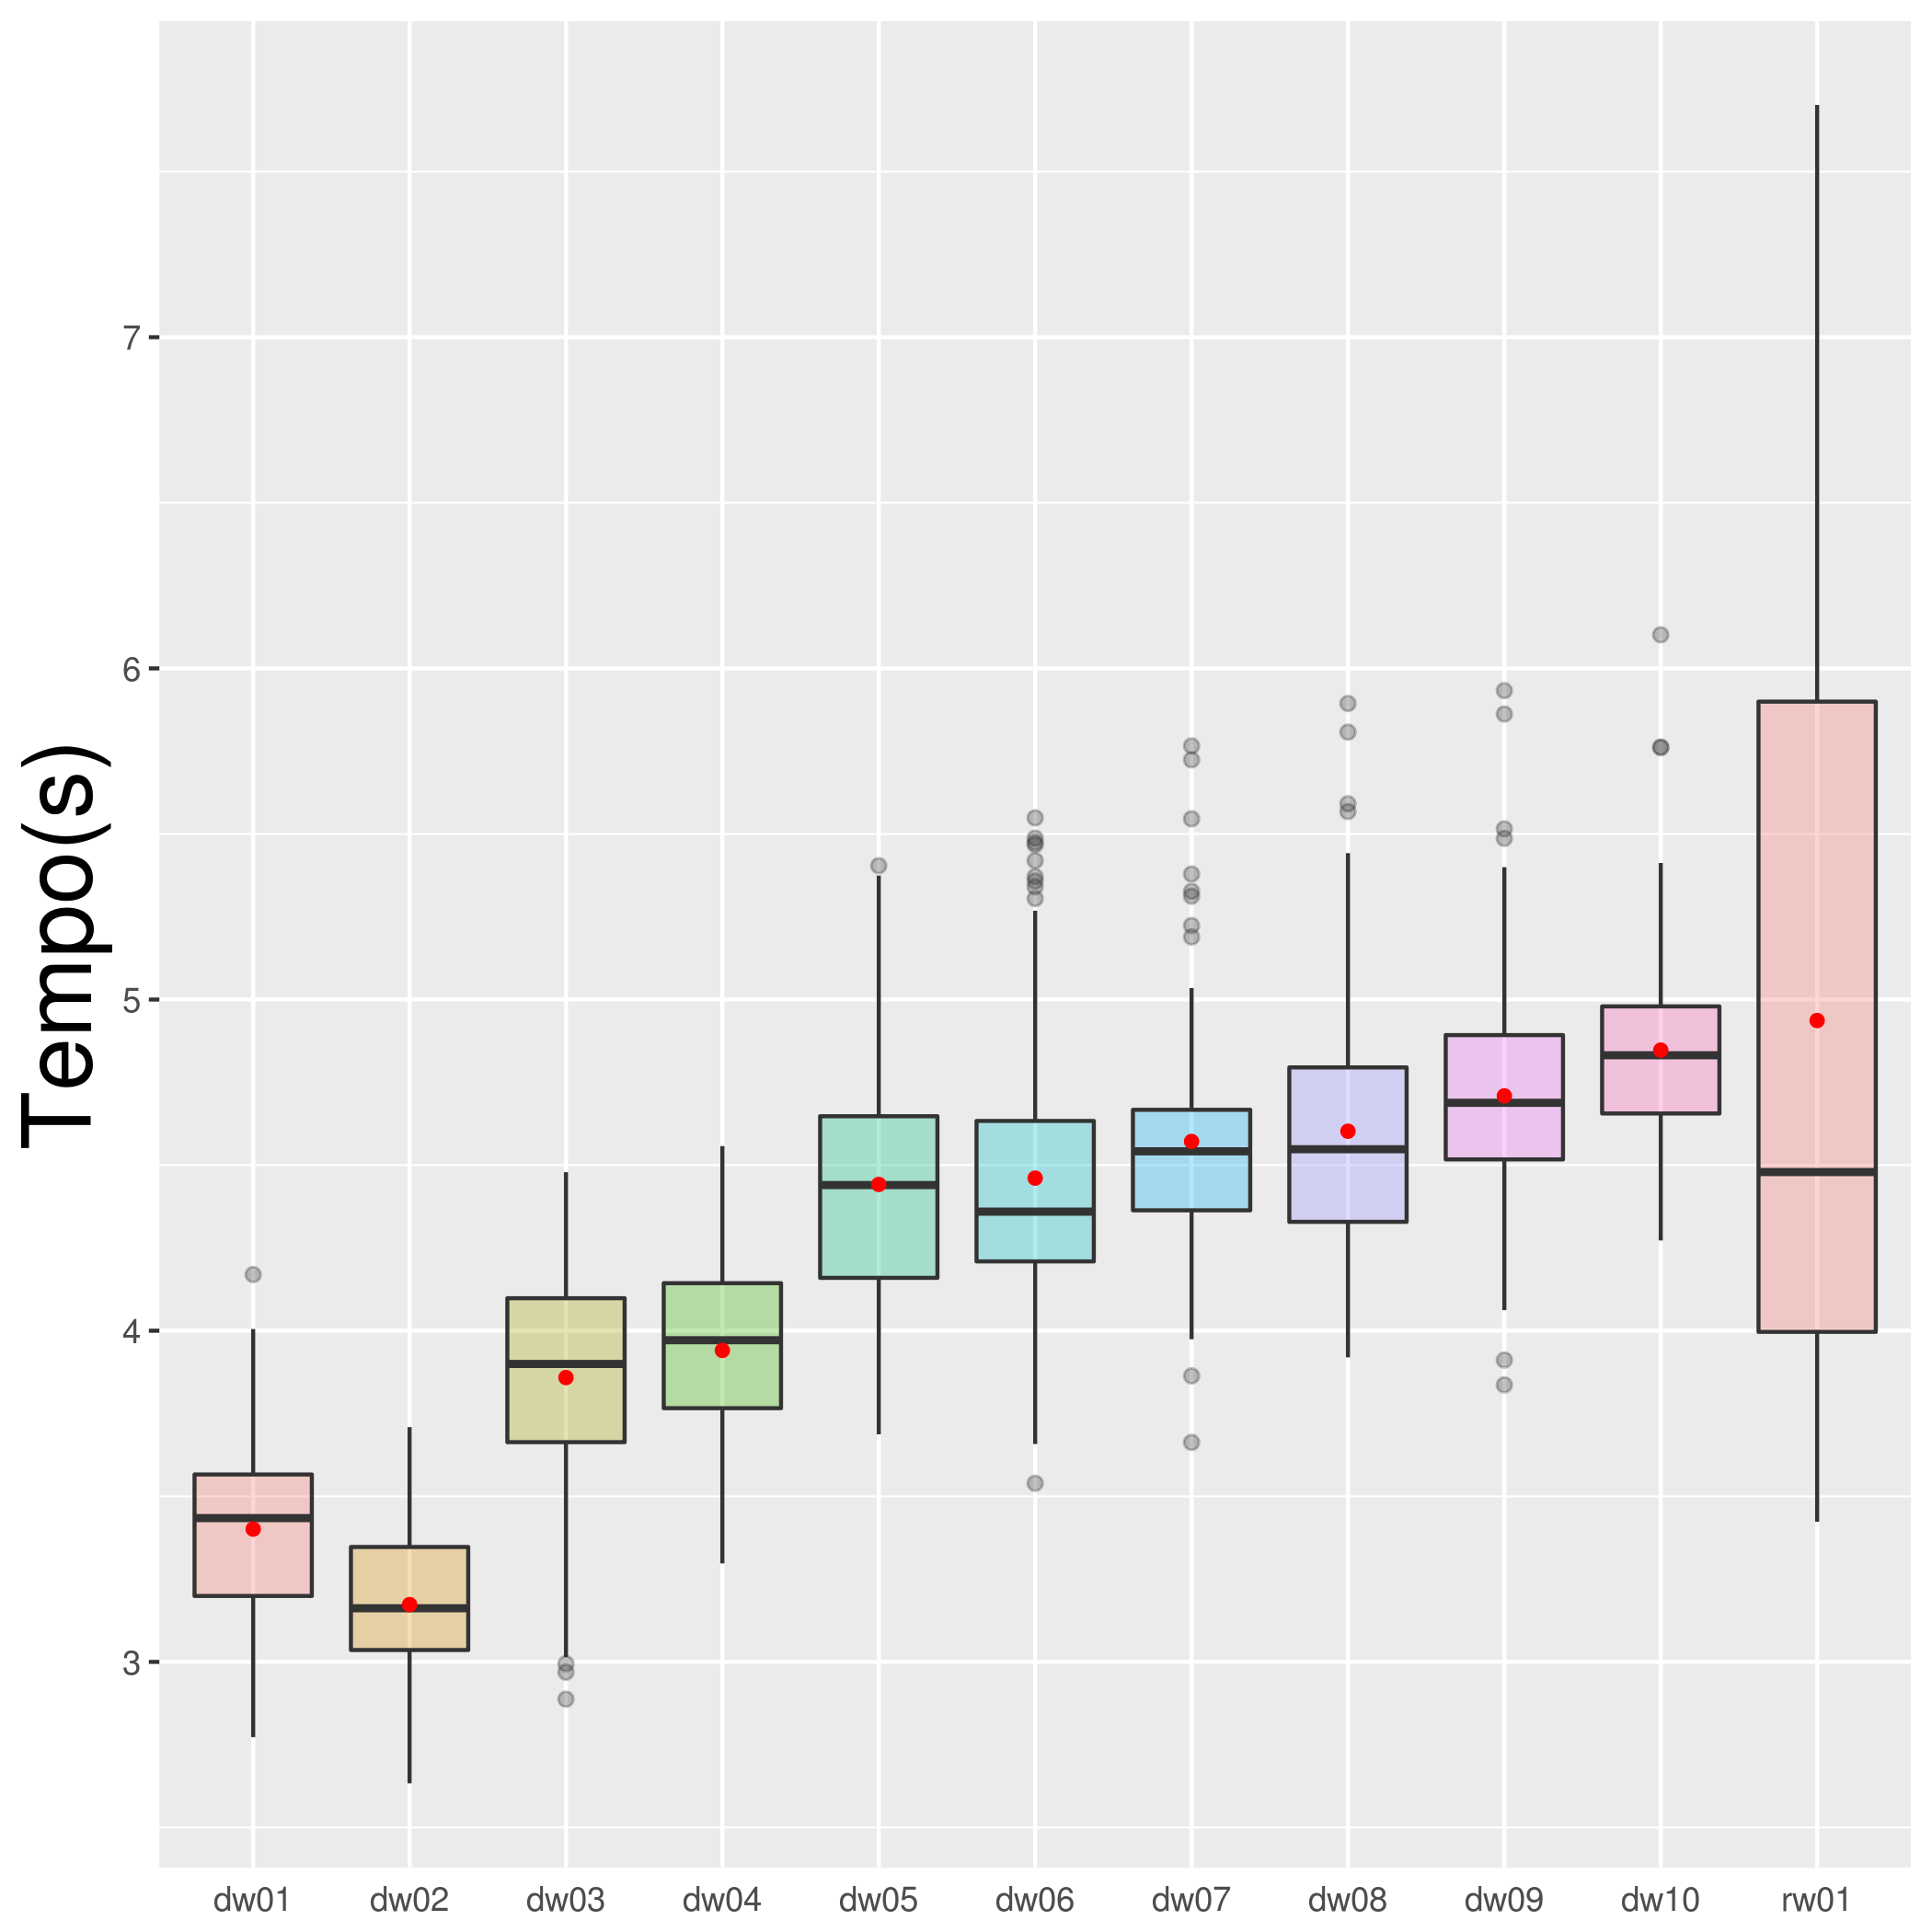
\includegraphics[scale=0.4]{figuras/dvnd/n1/time5.png}
        \label{fig:timeDvndRvnd_n1in5}
    }}%
    \caption{Tempos DVND e RVND das instâncias 4 e 5 para $n=1$.}%
    \label{fig:timeDvndRvnd_n1in4_5}%
\end{figure}

\begin{figure}%
    \centering
    \subfloat[Instância 6]{{
        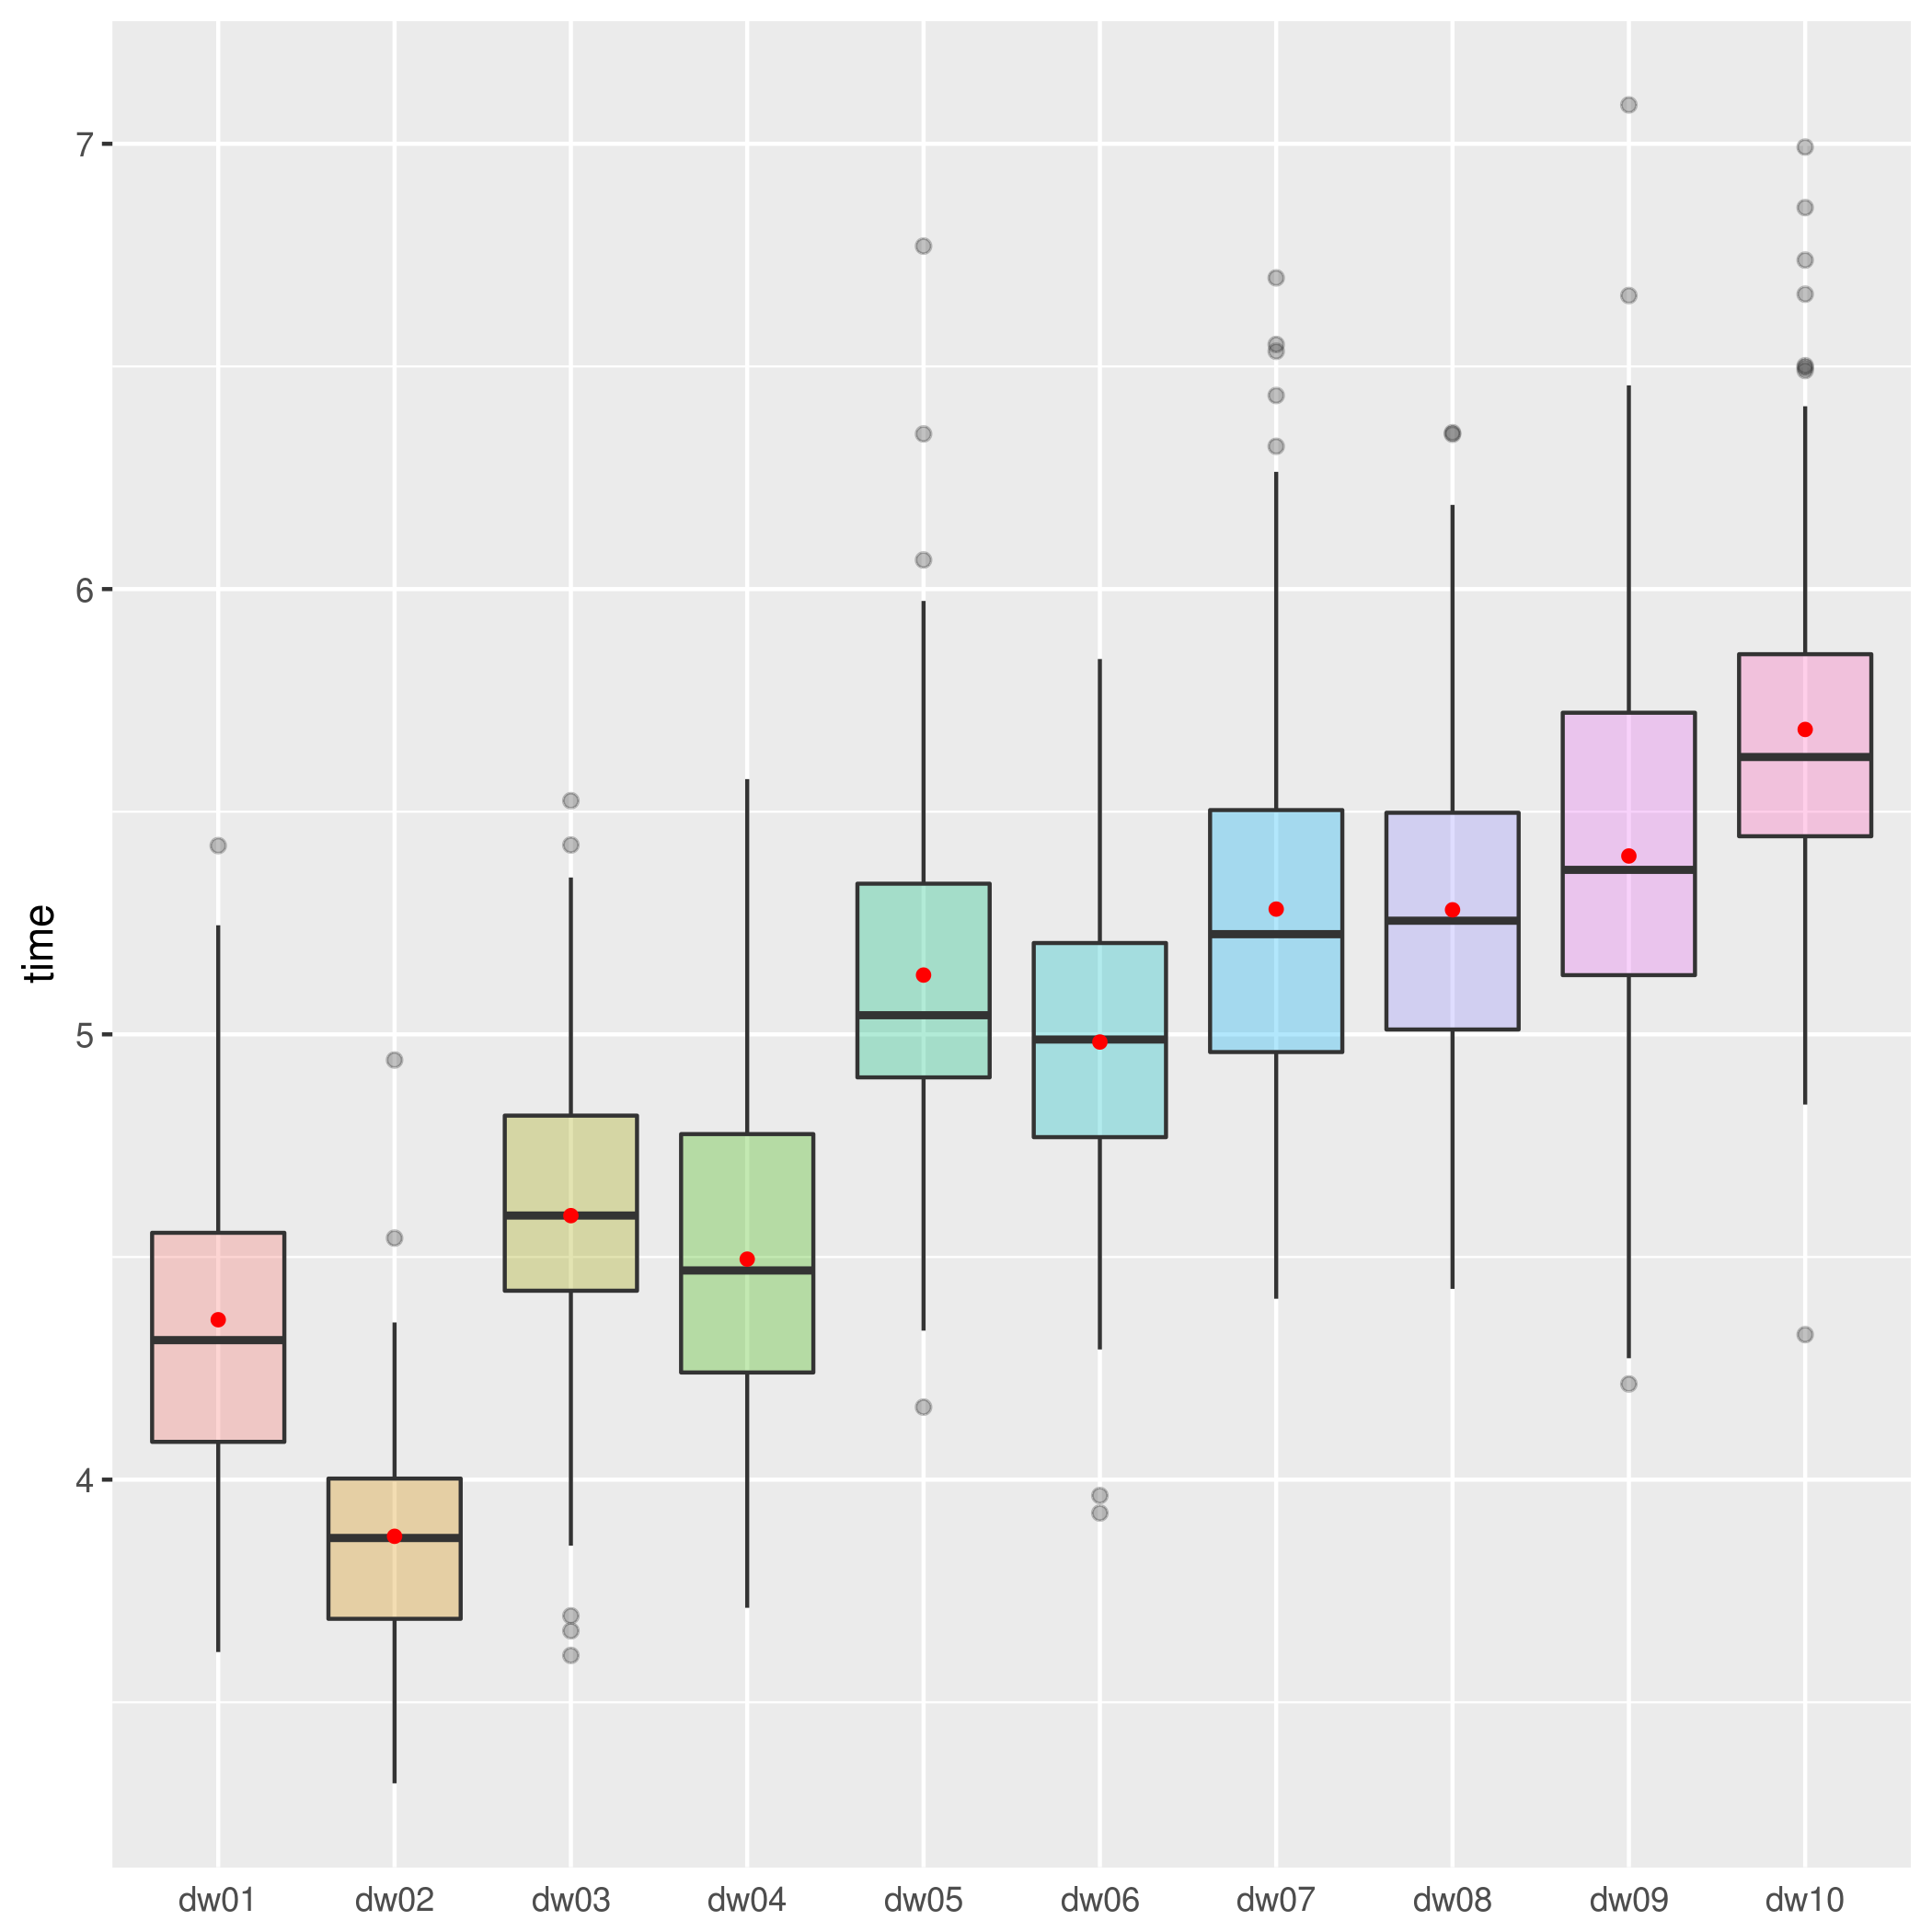
\includegraphics[scale=0.4]{figuras/dvnd/n1/time6.png}
        \label{fig:timeDvndRvnd_n1in6}
    }}%
    \qquad
    \subfloat[Instância 7]{{
        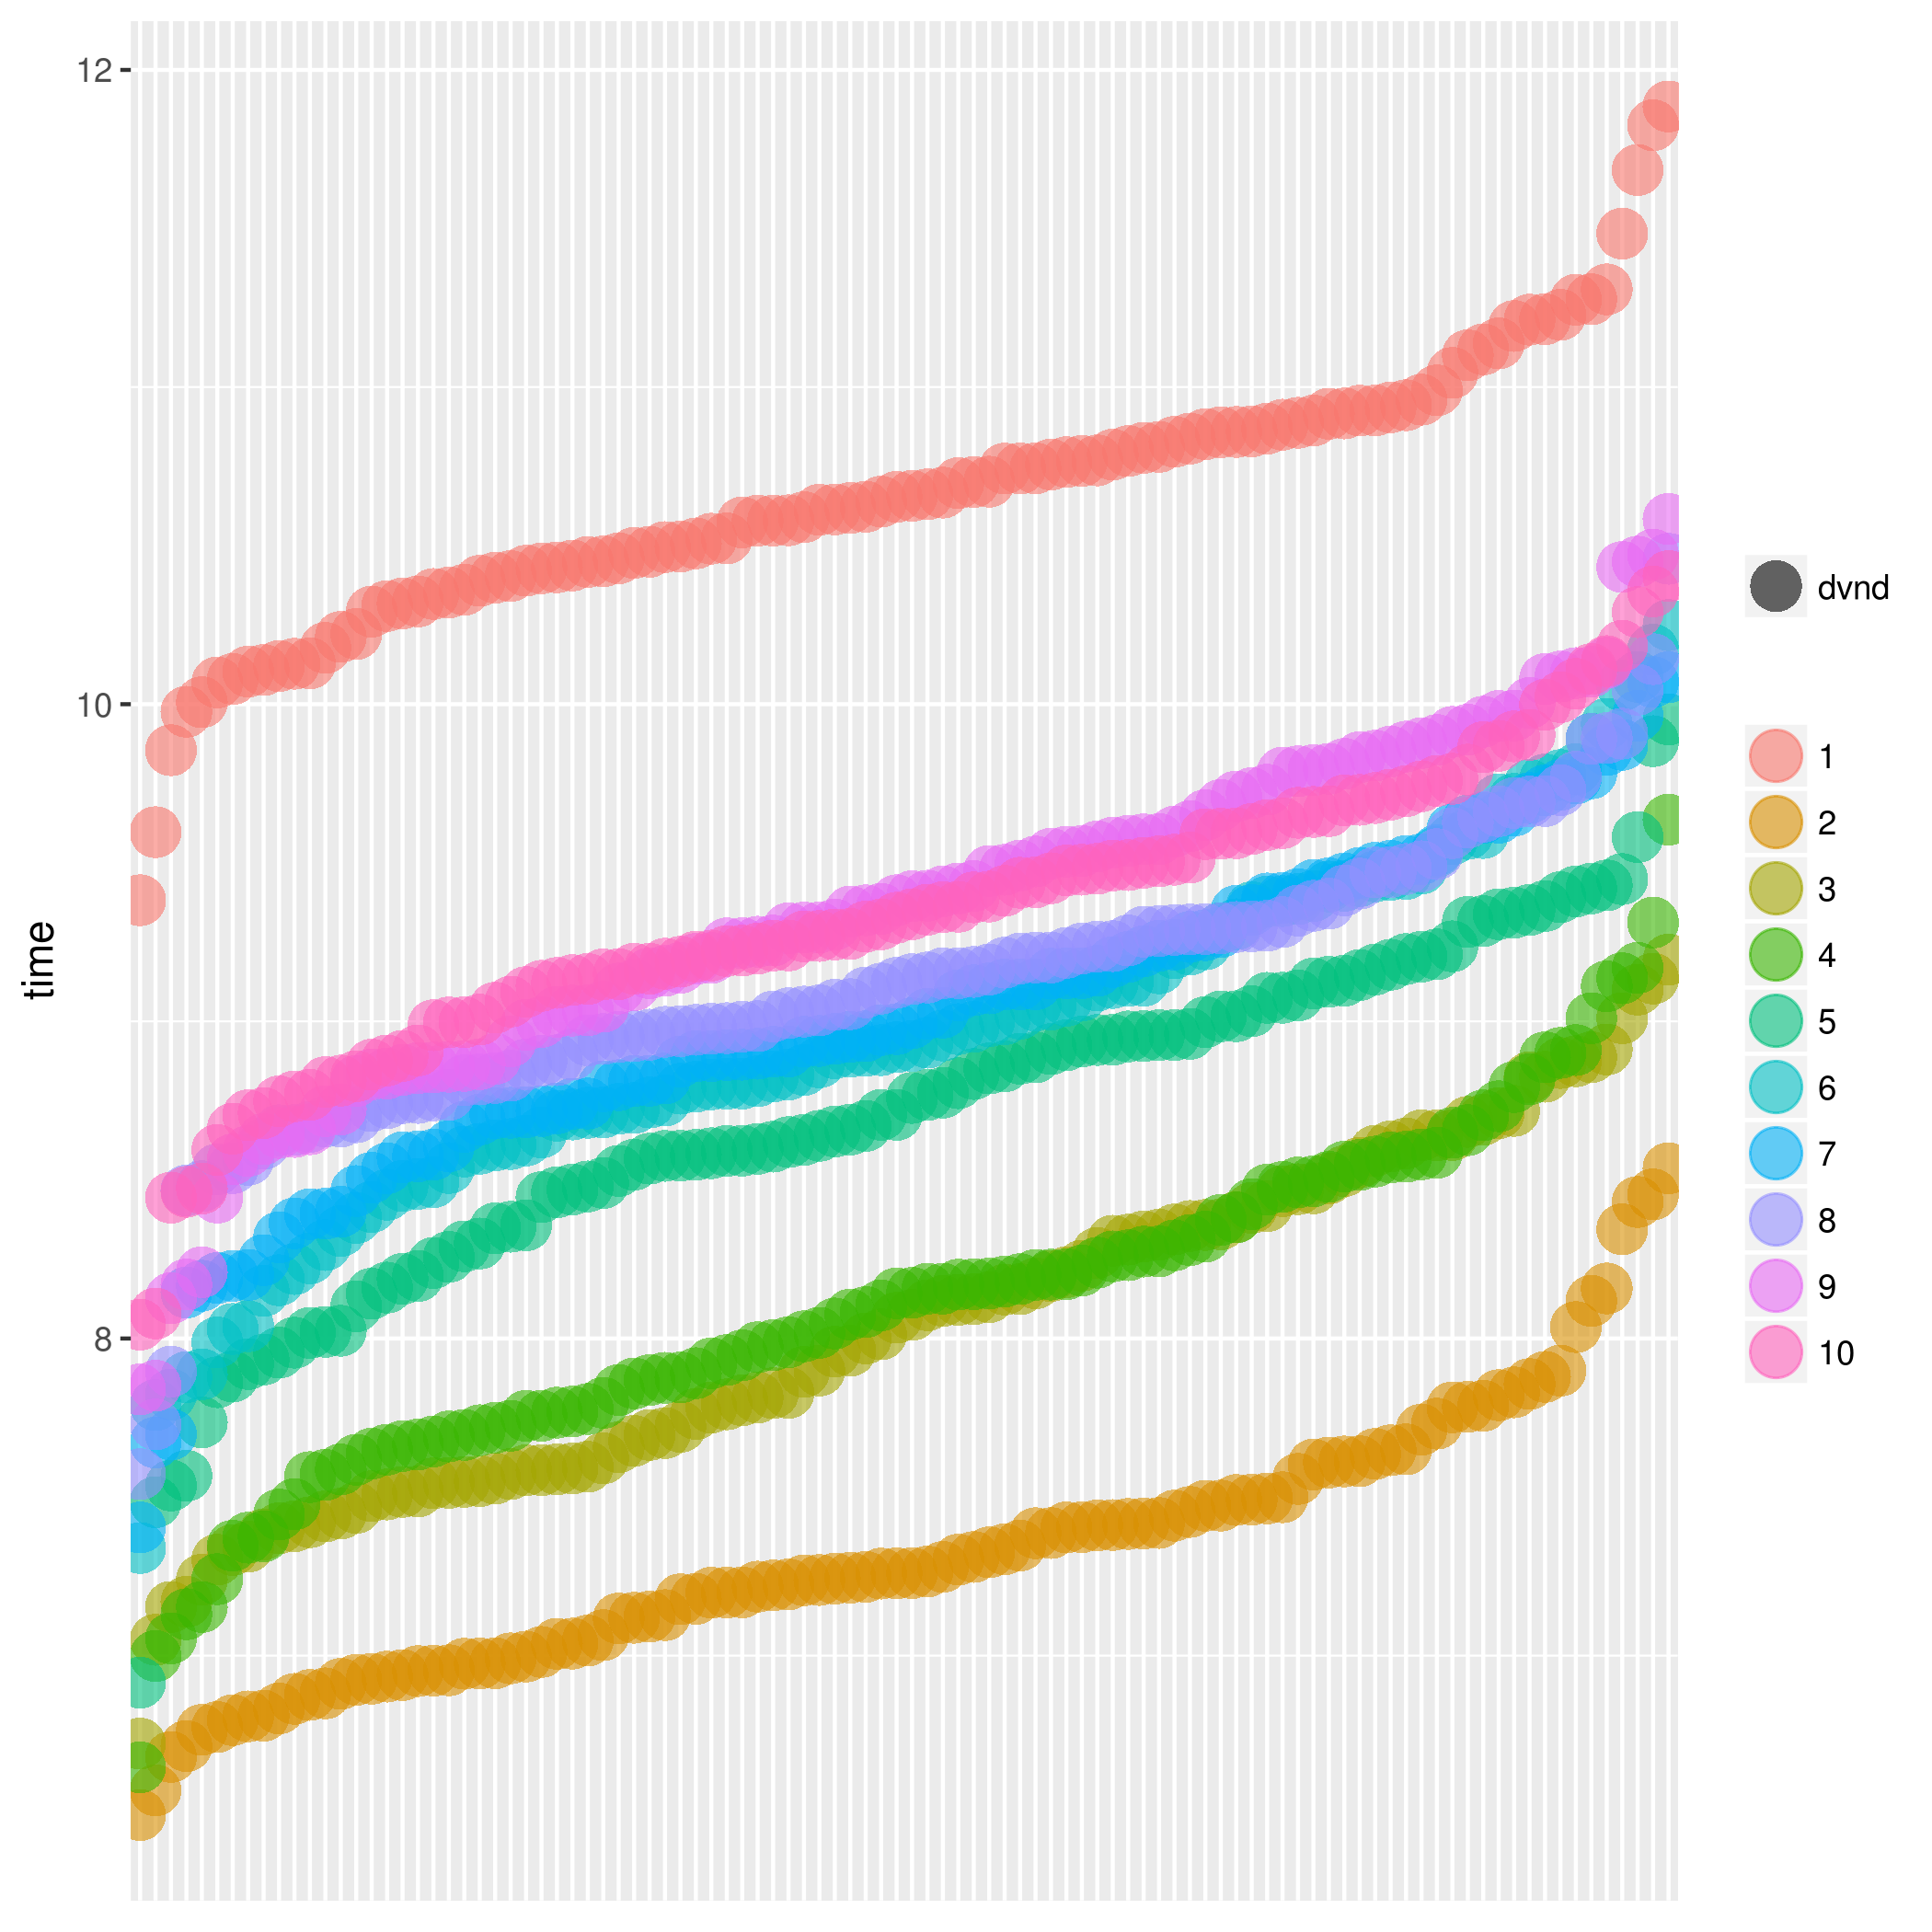
\includegraphics[scale=0.4]{figuras/dvnd/n1/time7.png}
        \label{fig:timeDvndRvnd_n1in7}
    }}%
    \caption{Tempos DVND e RVND das instâncias 6 e 7 para $n=1$.}%
    \label{fig:timeDvndRvnd_n1in6_7}%
\end{figure}
